\documentclass{beamer}
\setbeameroption{show notes}


\mode<presentation>
{
\usetheme{Pittsburgh}      % Madrid, Montpellier, Pittsburgh, Rochester, boxes
\usecolortheme{dove} 	% beaver, crane, dolphin, dove, lily, orchid, seagull, seahorse
\usefonttheme{default}  % or try serif, structurebold, ...
\setbeamertemplate{navigation symbols}{}
\setbeamertemplate{caption}[numbered]
}

\usepackage[portuguese]{babel}
\usepackage[utf8x]{inputenc}
\usepackage{multirow}
\usepackage{ragged2e}
\usepackage{textpos}
\usepackage[export]{adjustbox}
\usepackage{caption}
\justifying
\usepackage{pifont}
\newcommand{\xmark}{\ding{55}}%
\usepackage{tikz}
\usepackage[skins]{tcolorbox}
\usetikzlibrary{arrows,positioning} 
\usetikzlibrary{matrix}
\usetikzlibrary{fadings,shapes,arrows,chains,backgrounds,calc,arrows,arrows.meta,shadows,shapes.geometric, fit, positioning, circuits.logic.US, circuits, decorations.markings, arrows.meta}
\usepackage{tabularx}
\usepackage{booktabs}

\definecolor{lavenderblue}{rgb}{0.8, 0.8, 1.0}
\definecolor{aurometalsaurus}{rgb}{0.43, 0.5, 0.5}
\definecolor{bluegray}{rgb}{0.4, 0.6, 0.8}
\definecolor{glaucous}{rgb}{0.38, 0.51, 0.71}
\definecolor{coolblack}{rgb}{0.0, 0.18, 0.39}

\setlength{\parindent}{0.5cm}
%%%%%%%%%%%%%%%%%%%%%
% Títulos e etc
\title[Apresentação Final]{Co-processador da Transformada para o Codificador de Vídeo AV1}
\subtitle{Apresentação Final}
\author[M. Inocêncio]{Miguel Inocêncio}
\institute[UA]{Universidade de Aveiro\\ 
				Instituto de Telecomunicações}
\date{18/12/2019}
%\titlegraphic{
\includegraphics[height=1.5cm]{../ua.jpg}\includegraphics[height=1.5cm]{../IT.png}}

\begin{document}

%%%%%%%%%%%%%%%%%%%%%
% Página Inicial
\begin{frame}
	\titlepage
\end{frame}

%%%%%%%%%%%%%%%%%%%%%
% Table of Contents
\begin{frame}{Conteúdos}
	\tableofcontents
\end{frame}

%%%%%%%%%%%%%%%%%%%%%%
% Introdução
\section{Introdução}

\begin{frame}
	\frametitle{Consumo de Vídeo}
       \begin{columns}
              \column{\textwidth}
                     \begin{figure}[h]
                            \centering
                            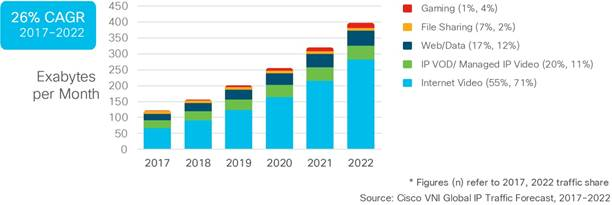
\includegraphics[width=\textwidth]{Figures/cisco.jpg}
                            \caption{Previsões da \emph{Cisco} para evolução de tráfico IP}
                            \label{fig:cisco}
                     \end{figure}
       \end{columns}
\end{frame}

\note[itemize]{
       \item Consumo de vídeo tem vindo a aumentar exponencialmente
       \item A Cisco prevê que para 2022 82\% do tráfico IP esteja dedicado à vizualização de vídeo
}

\begin{frame}
       \frametitle{Necessidade de Compressão de Vídeo}
       \begin{figure}[h]
              \centering
              \begin{tikzpicture}
    \makeatletter
    \tikzset{   len/.style={<->, line width=0.3mm, >=stealth'},
                to/.style={->, line width=0.8mm, >=stealth'},
                database/.style={
                    path picture={
                        \draw[very thick] (0, 1.5*\database@segmentheight) circle [x radius=\database@radius,y radius=\database@aspectratio*\database@radius];
                        \draw[very thick] (-\database@radius, 0.5*\database@segmentheight) arc [start angle=180,end angle=360,x radius=\database@radius, y radius=\database@aspectratio*\database@radius];
                        \draw[very thick] (-\database@radius,-0.5*\database@segmentheight) arc [start angle=180,end angle=360,x radius=\database@radius, y radius=\database@aspectratio*\database@radius];
                        \draw[very thick] (-\database@radius,1.5*\database@segmentheight) -- ++(0,-3*\database@segmentheight) arc [start angle=180,end angle=360,x radius=\database@radius, y radius=\database@aspectratio*\database@radius] -- ++(0,3*\database@segmentheight);
                    },
                    minimum width=2*\database@radius + \pgflinewidth,
                    minimum height=3*\database@segmentheight + 2*\database@aspectratio*\database@radius + \pgflinewidth,
                },
                database segment height/.store in=\database@segmentheight,
                database radius/.store in=\database@radius,
                database aspect ratio/.store in=\database@aspectratio,
                database segment height=0.1cm,
                database radius=0.25cm,
                database aspect ratio=0.35
            }

    \path[fill overzoom image={Figures/cat.jpg}] (0,0) node[minimum width=0.5\textwidth, minimum height=0.4\textheight, anchor=south west] (cat) {} rectangle (0.5\textwidth,0.4\textheight) {};
        \draw [len] ([xshift=-2mm] cat.south west) -- ([xshift=-2mm] cat.north west);
            \node at (cat.west) [rotate=90, yshift=5mm, font={\bfseries\large}] {720 px};
        \draw [len] ([yshift=2mm] cat.north west) -- ([yshift=2mm] cat.north east);
            \node at (cat.north) [yshift=5mm, font={\bfseries\large}] {1280 px};

    \node[database, label=below:24 GB, font={\bfseries\large}, database radius=1cm,database segment height=0.5cm, right=2cm of cat.east] (db) {};
        \draw[to] ([xshift=1mm]cat.east) -- ([xshift=-1mm]db.west) node [midway,above] {5 min.};
\end{tikzpicture}
       \end{figure}
\end{frame}

\note[itemize]{
       \item Enorme quantidade de dados gerados com a captura ou criação de vídeo
       \item Vídeo HD a 30 frames por segundo num espaço RGB de 8 bits por cor ocuparia 24GB em 5 minutos
       \item Para as resoluções que se desejam hoje em dia este problema seria ainda mais grave
       \item Necessidade de reduzir quantidade de informação precisa para reproduzir um vídeo
}

\begin{frame}
       \frametitle{Codificação de Vídeo}
       \begin{center}
              \Large Remoção de informação de sequência de imagens, mantendo a capacidade de reprodução
       \end{center}
\end{frame}

\note[itemize]{
       \item Levou ao conceito de codificação de vídeo
}

\begin{frame}
       \frametitle{Evolução da Codificação de Vídeo}
       \begin{figure}[h]
              \centering
              \begin{tikzpicture} [y=1cm]
    \makeatletter
    \tikzset{   len/.style={<->, line width=0.3mm, >=stealth'},
                to/.style={->, line width=0.8mm, >=stealth'}
            }

    \foreach \x in {0,0.6,1.2,1.8}
        \draw[fill=green!80!black, draw=black] (0,\x) rectangle (3,\x+0.3);
    \foreach \x in {0.3,0.9,1.5,2.1}
        \draw[fill=red!80!black, draw=black] (0,\x) rectangle (3,\x+0.3);
    \node at (1.5,-0.2) [below, font={\bfseries\large}] {1940};

    \draw[to] (3.2,1.2) -- (4.5,1.2);
    \node[inner sep=0pt, anchor=west] at (4.7,1.2) (av1l) {
\includegraphics[width=3cm]{Figures/av1.png}};
    \node at (6.1,-0.2) [below, font={\bfseries\large}] {2018};
\end{tikzpicture}
       \end{figure}
\end{frame}

\note[itemize]{
       \item Em prática desde os anos 40 com o interlaced scanning das televisões de raios catódicos
       \item Evolução do vídeo levou à evolução dos métodos de compressão (aumento da complexidade)
       \item Alliance for Open Media Video One ou AV1 apresenta grandes taxas de compressão, a custo de elevada complexidade
       \item Necessidade de software optimizado e arquiteturas de hardware eficientes
}

%%%%%%%%%%%%%%%%%%%%%%
% Sistemas de Codificação de Vídeo
\section{Sistemas de Codificação de Vídeo}
\begin{frame}[c]
       \begin{center}
              \Huge \textbf{Sistemas de Codificação de Vídeo}
       \end{center}
\end{frame}

\note[itemize]{
       \item Operação feita por codec
       \item Composto por codificador e descodificador
       \item Tem como princípio base a remoção de dados previsíveis, ou redundantes
}

\begin{frame}
       \frametitle{Redundâncias}
       \begin{columns}
              \column{0.5\textwidth}
                     \begin{figure}[h]
                            \centering
                            \begin{tikzpicture}[scale=0.7,>=triangle 60]
\tikzset{
    a/.style={->},
}    
    \draw [fill=lightgray] (0,0) rectangle (1,5);
    \draw [fill=lightgray] (1,4) rectangle (9,5);
    \draw[step=1cm,black,very thin] (0,0) grid (5,5);
    \draw[step=1cm,black,very thin] (5,4) grid (9,5);

    \node at (1.5,4.5) {A};
    \node at (2.5,4.5) {B};
    \node at (3.5,4.5) {C};
    \node at (4.5,4.5) {D};
    \node at (5.5,4.5) {E};
    \node at (6.5,4.5) {F};
    \node at (7.5,4.5) {G};
    \node at (8.5,4.5) {H};

    \node at (0.5,4.5) {I};
    \node at (0.5,3.5) {J};
    \node at (0.5,2.5) {K};
    \node at (0.5,1.5) {L};
    \node at (0.5,0.5) {M};

    \draw [a] (8,4) --(4,0);
    \draw [a] (7,4) --(3,0);
    \draw [a] (6,4) --(2,0);
    \draw [a] (5,4) --(1,0);
    \draw [a] (4,4) --(1,1);
    \draw [a] (3,4) --(1,2);
    \draw [a] (2,4) --(1,3);
\end{tikzpicture}
                            \caption*{Espaciais}
                     \end{figure}
                     \begin{figure}[h]
                            \centering
                            \begin{tikzpicture}[scale=0.75]    
    \coordinate (ycenter) at (2,3);
    \node[align=center] at (ycenter.north) {\textbf{Y}};
    \fill[gray!40] (0,0) rectangle (1,1);
    \fill[gray!70] (1,0) rectangle (2,1);
    \fill[gray!40] (2,0) rectangle (3,1);
    \fill[gray!70] (3,0) rectangle (4,1);
    \fill[gray!70] (0,1) rectangle (1,2);
    \fill[gray!40] (1,1) rectangle (2,2);
    \fill[gray!70] (2,1) rectangle (3,2);
    \fill[gray!40] (3,1) rectangle (4,2); 
    
    \coordinate (ccenter) at (7,3);
    \node[align=center] at (ccenter.north) {\textbf{Cb/Cr}};
    \fill[blue!80!black] (5,0) rectangle (6,1);
    \fill[blue!80!black] (6,0) rectangle (7,1);
    \fill[pink] (7,0) rectangle (8,1);
    \fill[pink] (8,0) rectangle (9,1);
    \fill[blue!80!black] (5,1) rectangle (6,2);
    \fill[blue!80!black] (6,1) rectangle (7,2);
    \fill[pink] (7,1) rectangle (8,2);
    \fill[pink] (8,1) rectangle (9,2);

\end{tikzpicture}
                            \caption*{Psico-Visuais}
                     \end{figure}
              \column{0.5\textwidth}
                     \begin{figure}[h]
                            \centering
                            \begin{tikzpicture}[scale=.7,every node/.style={minimum size=1cm},on grid,>=triangle 60]
		
    %slanting: production of a set of n 'laminae' to be piled up. N=number of grids.
    \begin{scope}[
            yshift=-83,every node/.append style={
            yslant=0.5,xslant=-1},yslant=0.5,xslant=-1
            ]
        % opacity to prevent graphical interference
        \fill[white,fill opacity=0.9] (0,0) rectangle (5,5);
        \draw[blue!40!black,very thick] (0,0) rectangle (5,5);%marking borders
        \filldraw[blue!30] (0.5,0.5) rectangle (1.5,1.5);
        \draw[gray, dashed] (0.5,1.5) -- (3.42,4.42);
        \draw[gray, dashed] (1.5,0.5) -- (4.42,3.42);
        \draw[gray, dashed] (0.5,0.5) -- (3.42,3.42);
        \draw[gray, dashed] (1.5,1.5) -- (4.42,4.42);
        %Idem as above, for the n-th grid:
    \end{scope}
    
    \begin{scope}[
    	    yshift=0,every node/.append style={
    	    yslant=0.5,xslant=-1},yslant=0.5,xslant=-1
            ]
        \fill[white,fill opacity=.9] (0,0) rectangle (5,5);
        \draw[black,very thick] (0,0) rectangle (5,5);

        \draw[blue!30] (0.5,0.5) rectangle (1.5,1.5);
        \filldraw[gray] (2.5,3) rectangle (3.5,4);

        \draw[->] (0.5,0.5) -- (2.5,3);
    \end{scope}

    \draw[-latex,thick](5.8,0)node[right]{Reference Frame}
    to[out=180,in=90] (3.4,-1);

    \draw[-latex,thick] (5.8,3) node[right]{Present Frame}
         to[out=180,in=90] (3.4,2);

    \draw[-latex,thick] (-5.5,2.2) node[left]{Motion Vector}
    to [out=0,in=180](-0.22,1.5);
\end{tikzpicture}
                            \caption*{Temporais}
                     \end{figure}
                     \begin{figure}[h]
                            \centering
                            \begin{tikzpicture}[iv/.style={draw,fill=red!50,circle,minimum size=20pt,inner
    sep=0pt,text=black},ev/.style={draw,fill=yellow,rectangle,minimum
    size=20pt,inner sep=0pt,text=black},scale=0.3, every node/.style={transform shape}]
    \node[iv]{31}
      child {node[iv]{18}
             child {node[iv]{11}  
                    child {node[iv]{6}
                           child {node[iv]{3}
                                  child {node[ev]{E(1)}}
                                  child {node[ev]{C(2)}}
                                 }
                           child {node[ev]{B(3)}}
                          }
                    child {node[ev]{D(5)}}
                    }
             child [missing]
             child {node[iv]{7}
             child {node[ev]{A(4)}}
             child {node[ev]{G(3)}}
                   }
            edge from parent node[above]{O}        
            }
      child [missing]
      child [missing]
      child {node[iv]{13}
             child {node[ev]{F(6)}}
             child {node[ev]{H(7)}}
            };
\end{tikzpicture}
                            \caption*{Código}
                     \end{figure}
       \end{columns}
\end{frame}

\note[itemize]{
       \item Apesar da evolução, os princípios de base continuam os mesmos
       \item 4 tipos de redundâncias, a maioria causadas pela interpretação do olho humano
       \item Espaciais referentes à proximidade de pixeis proximos
       \item Temporais referentes à semelhança de pixeis em imagens consecutivas
       \item Psicovisuais referentes à perceção mais baixa da cor ou de detalhes
       \item Código, não sendo referente à imagem ou perceção, mas à representação dos símbolos em domínio digital
       \item Estas redundâncias são exploradas em vários estágios de um codificador de vídeo
}

\begin{frame}
       \frametitle{Modelo Básico do Codificador}
       \begin{figure}[h]
              \centering
              \begin{tikzpicture}[%
    >=triangle 60,              % Nice arrows; your taste may be different
    start chain=going right,    % General flow is top-to-bottom
    node distance=2.5cm,          % Global setup of box spacing
    every join/.style={norm},   % Default linetype for connecting boxes
    scale=0.7, every node/.style={transform shape}
    ]

\tikzset{
    base/.style={draw, on chain, on grid, align=center},
    proc/.style={base, rectangle, text width=1.6cm, fill=black!15, minimum height=1.5cm, minimum width=1.5cm,font={\bfseries}},    
    frame/.style={base, minimum height=1.5cm, minimum width=2cm, fill=blue!10, thick},
    sub/.style={base, circle, inner sep=0pt, radius=0.4cm, fill=black!10, minimum height=3.5ex, font={\bfseries}},
    spot/.style={circle, inner sep=0pt, radius=0.4cm, minimum height=2mm, draw},
    edge rectangle/.style={ to path={ rectangle (\tikztotarget)}},
    % coord node style is used for placing corners of connecting lines
    coord/.style={coordinate, on chain, on grid, node distance=6mm and 40mm},
    % Arrows 
    fforw/.style={->, thick},
    fback/.style={->, thick, red!75!black},
    aref/.style={<->, dashed, black!50},
    % -------------------------------------------------
    % Connector line styles for different parts of the diagram
    cascaded/.style = {%
    general shadow = {%
      shadow scale = 1,
      shadow xshift = -1ex,
      shadow yshift = 1ex,
      draw,
      thick,
      fill = blue!40},
    general shadow = {%
      shadow scale = 1,
      shadow xshift = -.5ex,
      shadow yshift = .5ex,
      draw,
      thick,
      fill =blue!40},
    fill = blue!40, 
    draw,
    thick,
    minimum width = 2cm,
    minimum height = 1.5cm},
    base
}    

%% Top row
\node [frame] (inframe) {Input\\Frame};
    \node [coord] (ni1) {};    
    \node [coord, right=2mm of inframe.east] (ni2) {};
\node [sub, right=2cm of ni1] (sub) {-};
    \draw [fforw] (inframe) -- (sub);
\node [proc] (T) {T};
    \draw [fforw] (sub) -- (T);
\node [proc] (Q) {Q};
    \draw [fforw] (T) -- (Q);
\coordinate (rq) at ($(Q.east)+(4mm,0)$);
\node [proc, right=1cm of Q.east] (EC) {Entropy\\Coding};
    \draw [fforw] (Q) -- (EC);
\coordinate (out) at ($(EC.east)+(4mm,0)$);
%\path (EC) to node [yshift=-1em] {Encoded\\Bitstream} (out);
    \draw [fforw] (EC) -- (out);

%% Reference
\node [cascaded, below=5cm of inframe] (ref) {Reference\\Frames};

%% Intra
\node [proc, below=1.5cm of ni1] (intra) {Intra\\Coding};
    \coordinate (ni3) at (ni2 |- intra);    
    \draw [fforw] (ni3) -- (intra);

%% Inter    
\node [proc,right=of ref] (inter) {Inter\\Coding};
    \node [coord, below=4.5cm of ni2] (ni4) {};
    \draw [fforw] (ni2) -- (ni4) |- ($(inter.west)+(0,5mm)$);
    \draw [fforw] ($(ref.east)+(0,-5mm)$) -- ($(inter.west)+(0,-5mm)$);

%% Selector
\coordinate (rintra) at ($(intra.east)+(5mm,0)$);
\node [spot, below=1cm of rintra, fill=black] (sintra) {};
    \draw [thick] (intra.east) -- (rintra) |- (sintra.north);

\coordinate (rinter) at ($(inter.east)+(5mm,0)$);
\node [spot, above=1cm of rinter, fill=black] (sinter) {};
    \draw [thick] (inter.east) -- (rinter) |- (sinter.south);

\path (sintra) -- (sinter) coordinate [midway] (intraintermid);
\node [spot, at=(sub |- intraintermid)] (sel) {};
\draw [dashed] ($(sel)+(-4mm,3.3mm)$) arc (140:220:5mm);
    \draw [fforw] (sintra) -- (sel);
    \draw [fforw] (sel) -- (sub);

%% Lower Row    
\node [sub, below=3.7cm of sel] (add) {+};
    \draw [fback] (sel) -- (add);
\node [proc] (T1) {$\mathbf{T^{-1}}$};
    \draw [fback] (T1) -- (add);
\node [proc] (Q1) {$\mathbf{Q^{-1}}$};
    \draw [fback] (Q1) -- (T1);
\coordinate (rq1) at ($(Q1.east)+(4mm,0)$);
    \draw [fback] (rq) -- (rq1) |- (Q1);
\node [frame, below=7.4cm of inframe] (recframe) {Reconstructed\\Frame};
    \draw [fback] (add) -- (recframe);
\end{tikzpicture}
       \end{figure}
\end{frame}

\note[itemize]{
       \item Processo começa com frame de entrada que é dividido em blocos
       \item Estágio de predição Intra ou Inter
       \item Bloco previsto subtraído por original
       \item Transformada é o foco do trabalho
       \item Avalia componentes de frequência
       \item Quantização avalia coeficientes de maior relevância para reconstrução de imagem
       \item codificador de entropia organiza símbolos segundo códigos de comprimento variável
       \item Loop de feedback para restaurar imagem do descodificador para uso nos estágios de predição
       \item Unidade de controlo escolhe quais as ferramentas de codificação a usar
       \item Descodificador faz operação inversa
}

\begin{frame}
       \frametitle{Performance do AV1}
       \begin{figure}[htbp]
              \raggedright
              \begin{tikzpicture}[scale=0.5, every node/.style={scale=0.5}, >=triangle 60]
                     \draw[thick] (-0.5,0) -- (12,0) ;
                     \draw[thick,->] (0,-0.5) -- (0,6) node[midway, rotate=90, above, font={\bfseries}]{Average Relative Bitrate};
                     
                     \node at (2,0) [below, font={\bfseries}] (h264) {H.264};
                         \draw [line width=5mm, darkgray] (2,0) -- (2,5)node[font={\bfseries}, yshift=2.5mm]{100\%};
                     \node at (5,0) [below, font={\bfseries}] (h264) {H.265};
                         \draw [line width=5mm, darkgray] (5,0) -- (5,3.5)node[font={\bfseries}, yshift=2.5mm]{70\%};
                     \node at (8,0) [below, font={\bfseries}] (h264) {VP9};
                         \draw [line width=5mm, darkgray] (8,0) -- (8,3.2)node[font={\bfseries}, yshift=2.5mm]{68\%};
                     \node at (11,0) [below, font={\bfseries}] (h264) {AV1};
                         \draw [line width=5mm, coolblack] (11,0) -- (11,2.6)node[font={\bfseries}, yshift=2.5mm]{53\%};
                 \end{tikzpicture}
       \end{figure}
       \begin{table}[h]
              \raggedleft
              \begin{tabular}{ccc} \toprule
                     \multirow{2}{*}{\textbf{Codec}}     &      \multicolumn{2}{c}{\textbf{Encoding Time (s)}} \\
                     &    \textbf{2018}  &   \textbf{2019}  \\ \toprule
                     AV1            &    226 080        & 736 \\ \hline
                     H.265          &    \multicolumn{2}{c}{289} \\ \hline
                     VP9            &    \multicolumn{2}{c}{226} \\ \hline
                     H.264          &    \multicolumn{2}{c}{18} \\
                     \bottomrule
              \end{tabular}    
       \end{table}
\end{frame}

\note[itemize]{
       \item Processo complexo
       \item Agravado pela complexidade do codificador
       \item Quanto mais opções de codificação, melhor a performance de compressão, mas maior o tempo de operação
       \item AV1 apresenta grandes poupanças em bit savings a custo de elevados tempos de operação
       \item Melhorias até 30\% em relação ao HEVC ou VP9 (formatos de codificação recentes)
       \item Demora até 3 vezes mais para atingir a mesma distorção
       \item Melhoria ao longo dos anos com optimização do software
}

%%%%%%%%%%%%%%%%%%%%%%
% Transformadas
\section{Transformadas em Codificação de Vídeo}

\begin{frame}[c]
       \begin{center}
              \Huge \textbf{Transformadas em Codificação de Vídeo}\\
       \end{center}
\end{frame}

\note[itemize]{
       \item Avanço para o estudo do software de referência
       \item objetivo de perceber funcionamento interno do estágio da Transformada
       \item Objetivo do estágio é decomposição em componentes de frequência
}

\begin{frame}
       \frametitle{Interpretação com Imagens Base}
       \begin{figure}[h]
              \centering
              \begin{tikzpicture}[%
    >=triangle 60,              % Nice arrows; your taste may be different
    every join/.style={norm},   % Default linetype for connecting boxes
    scale=0.35, every node/.style={transform shape},
    x=1cm,
    y=1cm
    ]

    %% Imagem Original
    \foreach \x in {0,0.5,...,3.5}
        \foreach \y in {0,0.5,...,3.5}
            \pgfmathsetmacro\grays{\x*9+\y*11+10}
            \draw[fill=black!\grays] (\x,\y-7) rectangle (\x+0.5,\y-7.5);
    \node at (2,-8.5) [align=center, font={\bfseries\huge}] {Imagem\\Original};
    \node at (5,-5.5) [align=center, font={\bfseries\huge}] {$\mathbf{=}$};

    %% DC
    \foreach \x in {0,0.5,...,3.5}
        \foreach \y in {0,0.5,...,3.5}
            \draw[fill=black!50] (6+\x,\y) rectangle (\x+6.5,\y+0.5);
    \node at (8,-0.5) [align=center, font={\bfseries\huge}] {$\mathbf{\times 0.6}$};  

    %% Horizontal
    \foreach \x in {0,0.5,...,3.5}
        \foreach \y in {0,0.5,...,3.5}
            \pgfmathsetmacro\grays{abs(cos(\x/3.5*90+90))*50}
            \draw[fill=black!\grays] (11+\x,\y) rectangle (\x+11.5,\y+0.5);
    \node at (13,-0.5) [align=center, font={\bfseries\huge}] {$\mathbf{\times 0.1}$};

    \foreach \x in {0,0.5,...,3.5}
        \foreach \y in {0,0.5,...,3.5}
            \pgfmathsetmacro\grays{abs(cos(\x/3.5*180+90))*60}
            \draw[fill=black!\grays] (16+\x,\y) rectangle (\x+16.5,\y+0.5);
    \node at (18,-0.5) [align=center, font={\bfseries\huge}] {$\mathbf{\times 0.04}$};

    \foreach \x in {0,0.5,...,3.5}
        \foreach \y in {0,0.5,...,3.5}
            \pgfmathsetmacro\grays{(abs(cos(\x/3.5*360+90)))*60}
            \draw[fill=black!\grays] (21+\x,\y) rectangle (\x+21.5,\y+0.5);
    \node at (23,-0.5) [align=center, font={\bfseries\huge}] {$\mathbf{\times 0.02}$};

    %% Vertical
    \foreach \x in {0,0.5,...,3.5}
        \foreach \y in {0,0.5,...,3.5}
            \pgfmathsetmacro\grays{abs(cos(\y/3.5*90))*50}
            \draw[fill=black!\grays] (6+\x,-5+\y) rectangle (\x+6.5,\y-4.5);
    \node at (8,-5.5) [align=center, font={\bfseries\huge}] {$\mathbf{\times (-0.14)}$};  

    \foreach \x in {0,0.5,...,3.5}
        \foreach \y in {0,0.5,...,3.5}
            \pgfmathsetmacro\grays{abs(cos(\y/3.5*180+90))*60}
            \draw[fill=black!\grays] (6+\x,-10+\y) rectangle (\x+6.5,\y-9.5);
    \node at (8,-10.5) [align=center, font={\bfseries\huge}] {$\mathbf{\times 0.01}$};  

    \foreach \x in {0,0.5,...,3.5}
        \foreach \y in {0,0.5,...,3.5}
            \pgfmathsetmacro\grays{(abs(cos(\y/3.5*360+90)))*60}
            \draw[fill=black!\grays] (6+\x,-15+\y) rectangle (\x+6.5,\y-14.5);
    \node at (8,-15.5) [align=center, font={\bfseries\huge}] {$\mathbf{\times 0.01}$};  

    %% Intermediary    
    \foreach \x in {0,0.5,...,3.5}
        \foreach \y in {0,0.5,...,3.5}
            \pgfmathsetmacro\grays{abs(cos(\x/3.5*90+90)*cos(\y/3.5*90))*60}
            \draw[fill=black!\grays] (11+\x,\y-5) rectangle (\x+11.5,\y-4.5);
    \node at (13,-5.5) [align=center, font={\bfseries\huge}] {$\mathbf{\times (-0.08)}$};  

    \foreach \x in {0,0.5,...,3.5}
        \foreach \y in {0,0.5,...,3.5}
            \pgfmathsetmacro\grays{abs(cos(\x/3.5*180+90)*cos(\y/3.5*90))*60}
            \draw[fill=black!\grays] (16+\x,\y-5) rectangle (\x+16.5,\y-4.5);
    \node at (18,-5.5) [align=center, font={\bfseries\huge}] {$\mathbf{\times 0.0}$};  
                
    \foreach \x in {0,0.5,...,3.5}
        \foreach \y in {0,0.5,...,3.5}
            \pgfmathsetmacro\grays{abs(cos(\x/3.5*360+90)*cos(\y/3.5*90))*60}
            \draw[fill=black!\grays] (21+\x,\y-5) rectangle (\x+21.5,\y-4.5);
    \node at (23,-5.5) [align=center, font={\bfseries\huge}] {$\mathbf{\times 0.0}$};  

    \foreach \x in {0,0.5,...,3.5}
        \foreach \y in {0,0.5,...,3.5}
            \pgfmathsetmacro\grays{abs(cos(\x/3.5*90+90)*cos(\y/3.5*180+90))*60}
            \draw[fill=black!\grays] (11+\x,\y-10) rectangle (\x+11.5,\y-9.5);
    \node at (13,-10.5) [align=center, font={\bfseries\huge}] {$\mathbf{\times 0.0}$};  
    
    \foreach \x in {0,0.5,...,3.5}
        \foreach \y in {0,0.5,...,3.5}
            \pgfmathsetmacro\grays{abs(cos(\x/3.5*180+90)*cos(\y/3.5*180+90))*60}
            \draw[fill=black!\grays] (16+\x,\y-10) rectangle (\x+16.5,\y-9.5);
    \node at (18,-10.5) [align=center, font={\bfseries\huge}] {$\mathbf{\times 0.0}$};  
                    
    \foreach \x in {0,0.5,...,3.5}
        \foreach \y in {0,0.5,...,3.5}
            \pgfmathsetmacro\grays{abs(cos(\x/3.5*360+90)*cos(\y/3.5*180+90))*60}
            \draw[fill=black!\grays] (21+\x,\y-10) rectangle (\x+21.5,\y-9.5);    
    \node at (23,-10.5) [align=center, font={\bfseries\huge}] {$\mathbf{\times 0.0}$};  
            
            
    \foreach \x in {0,0.5,...,3.5}
        \foreach \y in {0,0.5,...,3.5}
            \pgfmathsetmacro\grays{abs(cos(\x/3.5*90+90)*cos(\y/3.5*360+90))*60}
            \draw[fill=black!\grays] (11+\x,\y-15) rectangle (\x+11.5,\y-14.5);
    \node at (13,-15.5) [align=center, font={\bfseries\huge}] {$\mathbf{\times 0.0}$};  

    \foreach \x in {0,0.5,...,3.5}
        \foreach \y in {0,0.5,...,3.5}
            \pgfmathsetmacro\grays{abs(cos(\x/3.5*180+90)*cos(\y/3.5*360+90))*60}
            \draw[fill=black!\grays] (16+\x,\y-15) rectangle (\x+16.5,\y-14.5);
    \node at (18,-15.5) [align=center, font={\bfseries\huge}] {$\mathbf{\times 0.0}$};  
                
    \foreach \x in {0,0.5,...,3.5}
        \foreach \y in {0,0.5,...,3.5}
            \pgfmathsetmacro\grays{abs(cos(\x/3.5*360+90)*cos(\y/3.5*360+90))*60}
            \draw[fill=black!\grays] (21+\x,\y-15) rectangle (\x+21.5,\y-14.5);    
    \node at (23,-15.5) [align=center, font={\bfseries\huge}] {$\mathbf{\times 0.0}$};  

    %\node at (15.5,2) [align=center, font={\bfseries\huge}] {$\mathbf{+}$};

    %\foreach \x in {0,0.5,...,3.5}
    %    \foreach \y in {0,0.5,...,3.5}
    %        \pgfmathsetmacro\grays{\y*20}
    %        \draw[fill=black!\grays] (16+\x,\y) rectangle (\x+16.5,\y+0.5);
    %\node at (18,-0.5) [align=center, font={\bfseries\huge}] {$\mathbf{\times 0.3}$};    


    
\end{tikzpicture}
       \end{figure}       
\end{frame}

\note[itemize]{
       \item Interpreção em imagens de base: um bloco original pode ser visto como a soma de diversos blocos com diferentes componentes de frequencia horizontal e/ou vertical
       \item Transformada vista como calculo da correlação entre imagem original e imagens base
       \item Conjunto de imagens base depende da transformada utilizada e do tamanho do bloco a transformar
       \item AV1 suporta blocos entre 4 e 64, incluíndo tamanhos rectangulares
}

\begin{frame}
       \frametitle{Transformadas em Codificação de Vídeo}
       \begin{columns}
              \column{0.5\textwidth}
                     \begin{figure}[h]
                            \begin{tikzpicture}[%
    >=triangle 60,              % Nice arrows; your taste may be different
    every join/.style={norm},   % Default linetype for connecting boxes
    scale=0.5, every node/.style={transform shape},
    x=1cm,
    y=1cm
    ]

    \draw[thick, step=0.5] (0,0) grid (4,4);
    \node at (2,6) [font={\huge}, anchor=south] (tc) {$\mathbf{T_{colunas}}$};
        \draw [very thick, ->] (tc) -- (2,4.1);
    \node at (-2,2) [font={\huge}, anchor=east] (tr) {$\mathbf{T_{linhas}}$};
        \draw [very thick, ->] (tr) -- (-0.1,2);
\end{tikzpicture}
                     \end{figure}
              \column{0.5\textwidth}
                     \begin{center}
                            \begin{itemize}
                                   \item Discrete Cosine Transform (DCT)
                                   \item Identity (IDTX)
                                   \item Asymmetric Discrete Sine Transform (ADST)
                                   \item \emph{Flip} - Asymmetric Discrete Sine Transform (Flip-ADST)
                            \end{itemize}
                     \end{center}
       \end{columns}
\end{frame}

\note[itemize]{
       \item Bloco de duas dimensões implica transformação a duas dimensões
       \item Transformada pode ser feita em duas operações separáveis para linhas e colunas ou vice-versa
       \item Operações denominadas por kernels da Transformada
       \item AV1 suporta 3 tipos: Identidade, DCT e ADST que pode ser calculada direta ou inversamente
       \item Kernels podem ser utilizados independentemente na vertical ou horizontal
}

\begin{frame}
       \frametitle{Transformada no AV1}
       \begin{figure}[h]
              \centering
              \begin{tikzpicture}[%
    >=triangle 60,              % Nice arrows; your taste may be different
    start chain=going below,    % General flow is top-to-bottom
    node distance=6mm and 40mm, % Global setup of box spacing
    every join/.style={norm},   % Default linetype for connecting boxes
    scale=0.5, every node/.style={transform shape},
    ]

\tikzset{
  base/.style={draw, on chain, on grid, align=center, minimum height=4ex},
  proc/.style={base, rectangle, text width=8em, fill=black!10},
  test/.style={base, diamond, aspect=2, text width=6em, fill=black!10},
  inout/.style={base,draw,trapezium,trapezium left angle=70,trapezium right angle=-70, fill=black!12},
  term/.style={proc, rounded corners},
  % coord node style is used for placing corners of connecting lines
  coord/.style={coordinate, on chain, on grid, node distance=6mm and 40mm},
  % nmark node style is used for coordinate debugging marks
  nmark/.style={draw, cyan, circle, font={\sffamily\bfseries}},
  % -------------------------------------------------
  % Connector line styles for different parts of the diagram
  norm/.style={->, draw},
  free/.style={->, draw, green3},
  cong/.style={->, draw, red3},
  it/.style={font={\itshape}}
}    
    
  \begin{scope}

    \node[inout, it] (start) {Bloco de Entrada};

    \node[proc, below=1.5cm of start] (get_col) {Ler coluna \texttt{i\_c}};
      \path (start.south) to node [near end, xshift=2em, text=coolblack] {\texttt{i\_c=0}} (get_col);
        \draw [->] (start.south) -- (get_col);
    
    \node[test, join] (ud_flip) {\texttt{ud\_flip}};      

    \node[proc] (T1) {$T$};
      \path (ud_flip.south) to node [near start, xshift=1em, text=red!80!black] {\texttt{0}} (T1);
          \draw [->] (ud_flip.south) -- (T1);
    
    \node[test, join] (lr_flip) {\texttt{lr\_flip}};   

    \node[proc] (store1) {Guardar coeficientes};
      \path (lr_flip.south) to node [near start, xshift=1em, text=red!80!black] {\texttt{0}} (store1);
            \draw [->] (lr_flip.south) -- (store1);

    \node[test, join, text width=7em] (i_col) {\texttt{i\_c == (size\_col - 1)}};

    \node [proc, right=11cm of get_col] (get_row) {Ler linha \texttt{i\_r}};
      \path (i_col.south) to node [near end, xshift=2em, yshift=-0.2em, text=coolblack] {\texttt{i\_r=0}} (get_row);
      \path (i_col.south) to node [near start, xshift=-1.5em, yshift=-3cm, text=red!80!black] {\texttt{true}} (get_row);
        \draw [->] (i_col.south) -- ++(0,-0.5) -- ++(6.3,0) -- ++(0,13) -| (get_row);

    \node[proc, join] (T2) {$T$};

    \node[proc, join] (store2) {Guardar coeficientes};

    \node[test, join, text width=7em] (i_row) {\texttt{i\_r == (size\_row - 1)}};

    \node[term,line width=0.8mm] (end) {Fim};      
      \path (i_row.south) to node [near start, xshift=-1.5em, yshift=0.1cm, text=red!80!black] {\texttt{true}} (end);
        \draw [->] (i_row.south) -- (end);

      \node[proc, right=of ud_flip] (flip_in) {Rodar vetor na vertical};
      \path (ud_flip.east) to node [near start, yshift=1em, text=red!80!black] {\texttt{1}} (flip_in);
          \draw [->] (ud_flip.east) -- (flip_in); 

      \node[coord, right=of T1] (T1_right) {};
      \path (flip_in.south) to node {} (T1_right);
        \draw [->] (flip_in.south) -- (T1_right) |- (T1);

      \node[proc, right=of lr_flip] (flip_in2) {Rodar vetor na horizontal};
      \path (lr_flip.east) to node [near start, yshift=1em, text=red!80!black] {\texttt{1}} (flip_in2);
          \draw [->] (lr_flip.east) -- (flip_in2); 

      \node[coord, right=of store1] (store1_right) {};
      \path (flip_in2.south) to node {} (store1_right);
        \draw [->] (flip_in2.south) -- (store1_right) |- (store1);

      \node[coord, left=of get_col] (get_col_left) {};
      \path (get_col_left) to node [yshift=0.5em, text=coolblack] {\texttt{i\_c+=1}} (get_col);
      \node[coord, left=of i_col] (i_col_left) {};
      \path (i_col.west) to node [yshift=-1em, text=red!80!black] {\texttt{false}} (i_col_left);
        \draw [->] (i_col.west) -- (i_col_left) |- (get_col_left) |- (get_col);

      \node[coord, left=of get_row] (get_row_left) {};
      \path (get_row_left) to node [yshift=0.5em, text=coolblack] {\texttt{i\_r+=1}} (get_row);
      \node[coord, left=of i_row] (i_row_left) {};
      \path (i_row.west) to node [yshift=-1em, text=red!80!black] {\texttt{false}} (i_row_left);
        \draw [->] (i_row.west) -- (i_row_left) |- (get_row_left) |- (get_row);
  \end{scope}        
  
  \begin{pgfonlayer}{background}
    % Left-top corner of the background rectangle
    \path (get_col_left.west |- get_col_left.north)+(-1.5cm,0.8cm) node (a11) {};
    % Right-bottom corner of the background rectanle
    \path (flip_in.east |- i_col.south)+(+0.2cm,-0.75cm) node (a21) {};
    % Draw the background
    \path[fill=black!2,rounded corners, draw=black!50, dashed]
      (a11) rectangle (a21);
    \path (a11 |- a21) node (a31) {};
    \path (a11) -- (a31) node[midway, rotate=90, yshift=-0.5cm] (mid_right) {\textbf{Transformada Vertical}};

    \path (get_row_left.west |- get_row_left.north)+(-0.2cm,0.8cm) node (a12) {};
    \path (flip_in.east |- i_col.south)+(+9.5cm,-0.75cm) node (a22) {};
    \path[fill=black!2,rounded corners, draw=black!50, dashed]
      (a12) rectangle (a22);
    \path (a22 |- a12) node (a32) {};
    \path (a22) -- (a32) node[midway, rotate=90, yshift=0.5cm] (mid_right) {\textbf{Transformada Horizontal}};
  \end{pgfonlayer}
\end{tikzpicture}
       \end{figure}
\end{frame}

\note[itemize]{
       \item Diagrama de operação das transformadas no AV1
       \item Começa com a transformada vertical (colunas)
       \item Blocos de flip usados quando se pretende fazer a transformação com Flip-ADST
       \item Quando todas as colunas foram transformadas, segue para a transformaçao linha a linha
       \item Kernels representados pelos blocos T
}


\end{document}